{\color{gray}\hrule}
\begin{center}
\section{Methodology}
\textbf{Systematic Procedure to Identify Papers}
\bigskip
\end{center}
{\color{gray}\hrule}
\begin{multicols}{2}
The research process started with the defintion of the topic together with our supervisor Professor Jean-Marc Pierson, together we decided to settle on creating a state fo the art review on the topic of Container and Cloud Computing, with a particular emphasis on energy consumption optimization. 
To begin with we defined a ``Search Pipeline'':

\begin{figure}[H]
    \centering
    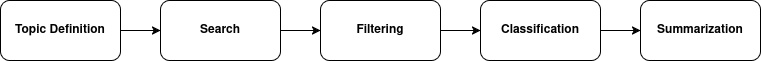
\includegraphics[width=\columnwidth]{flowchartTIR.png}
    \caption{Search Pipeline Flowchart}
    \label{fig:search_pipeline}
\end{figure}

This procedures allowed us to organize the work and have a standardized method of acceptance for navigating the papers. 
We also defined a search string with which we would start the search: ((energy OR resource) AND container).
We decided to expand the search also to resource since we noticed that many times better resource utilization leads to better dynamic power handling, hence lowering the amount of energy required to carry out a task.
Before starting with the research we also defined some acceptance criteria that would define whether a paper was going to be included in our survey or not. We defined the criteria as follows:

\begin{table}[H]
\centering
\begin{tabular}{c}
\hline
Direct Exclusion of Paper If \\ \hline
Work is not in English \\ 
Work is not a scientific paper \\ 
Work has less than 10 citations \\ 
Work is not about containers/cloud \\ \hline
\end{tabular}
    \caption{Exclusion Rules}
    \label{tab:Exclusion Rules}
\end{table}

Hence we proceeded with our search and we identified a total of 34 papers. That are divided as follows through the various publishers

\begin{figure}[H]
    \centering
    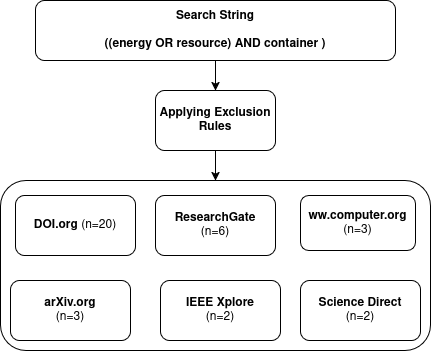
\includegraphics[width=\columnwidth]{sections/exportedPapers.png}
    \caption{Exported Papers}
    \label{fig:search_pipeline}
\end{figure}

To have an insight on the publication dates for the filtered papers, we can clearly visualize how the period between 2017 and 2019 was the most important for research in this field.

\begin{figure}[H]
    \centering
    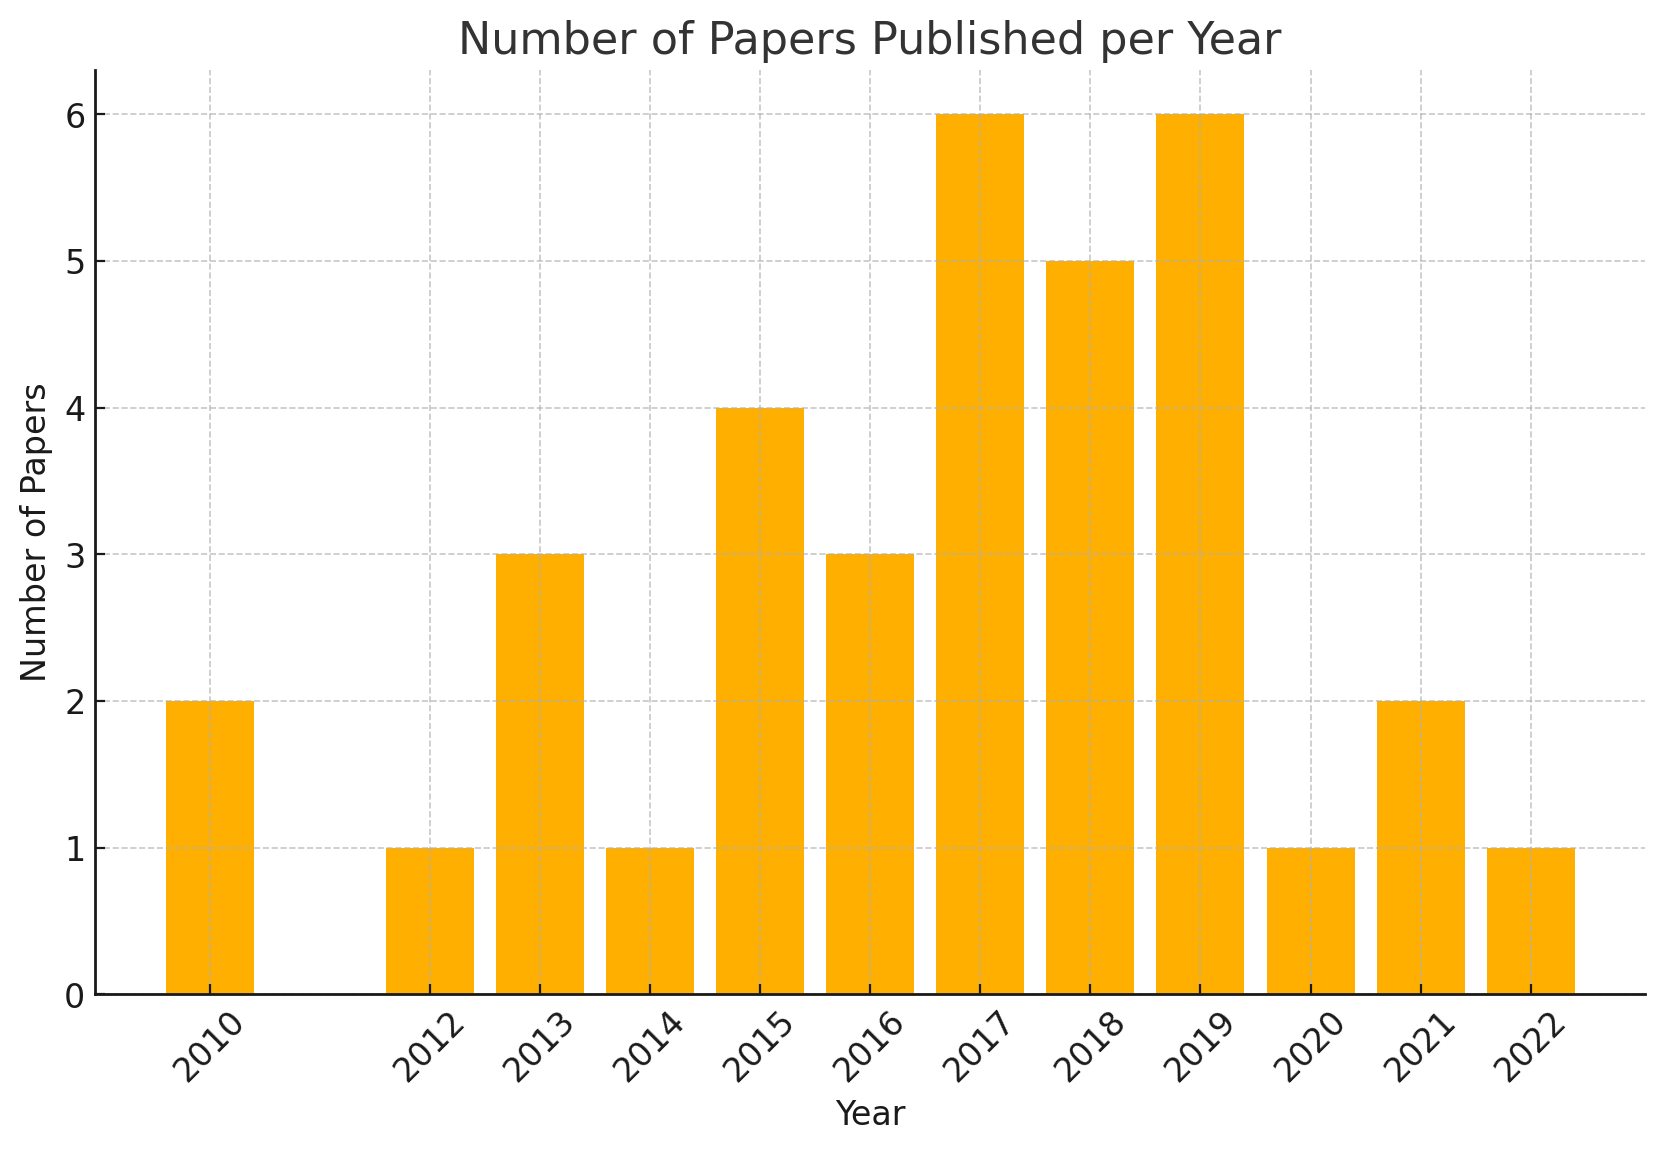
\includegraphics[width=\columnwidth]{papers_per_year.png}
    \caption{Papers per year}
    \label{fig:search_pipeline}
\end{figure}

At this point we could move to the classification step of our workflow. We decided to define the following  metrics

\begin{table}[H]
\centering
\begin{tabular}{c c}
\hline
Classification Categories\\ \hline
Optimization Technique \\ 
Target Level  \\ 
Scheduling Scope \\ 
Energy Strategy \\
Docker Awereness \\
\hline
\end{tabular}
    \caption{Paper Classification}
    \label{tab:Paper Classification}
\end{table}

The selected classification metrics capture the core technical dimensions of energy-aware scheduling research. Optimization Technique highlights the algorithmic strategy used. Target Level distinguishes whether the solution operates at the container, VM, or physical machine level. Scheduling Scope captures whether the approach is reactive, predictive, or concurrent. Energy Strategy defines the method used to reduce energy consumption, such as consolidation or renewable-aware placement. Finally, Docker Awareness situates each work in the context of containerization maturity, relevant for comparing approaches across technological shifts.

\end{multicols}

\begin{table}[H]
\centering
\footnotesize
\begin{tabular}{|p{3.8cm}|p{2.3cm}|p{1.6cm}|p{2.3cm}|p{2.2cm}|p{2cm}|}
\hline
\textbf{Paper (Short Title)} & \textbf{Optimization Algorithm} & \textbf{Target Level} & \textbf{Scheduling Scope} & \textbf{Energy Strategy} & \textbf{Docker Awareness} \\
\hline
Availability-Aware Scheduler\cite{alahmad_availability-aware_2018} (2018) & Greedy & Container, VM & Offline & Availability & Mature Docker\\
\hline
Renewable-Aware Scheduling\cite{kumar_renewable_2019} (2019)& Greedy & Container, VM & Reactive & Consolidation & Mature Docker \\
\hline
Concurrent Container Scheduling\cite{hu_concurrent_2020} (2020)& MCMF & Container & Concurrent & Consolidation & Mature Docker \\
\hline
GP Hyper-Heuristic for Containers\cite{tan_hybrid_2019} (2019)& Evolutionary & Container, VM & Online & Consolidation & Mature Docker \\
\hline
PSO-Based Container Consolidation\cite{shi_energy-aware_2018} (2018)& PSO & Container & Offline & Consolidation & Mature Docker \\
\hline
Energy-Efficient Container Framework\cite{piraghaj_framework_2015} (2015)& Greedy & Container, VM & Reactive & Consolidation & Early Docker \\
\hline
VM Consolidation Strategy\cite{carrega_energy-aware_2017} (2017)& Meta-Heuristic & VM & Online & Consolidation & Mature Docker \\
\hline
Predictive Resource Provisioning\cite{dabbagh_energy-efficient_2015} (2015)& Model-based  & VM & Predictive & Consolidation & Early-Docker \\
\hline
Dynamic VM Reallocation\cite{beloglazov_energy_2010} (2010) & Greedy & VM & Online & Consolidation & Pre-Docker \\
\hline
Autonomic Container Management\cite{barna_delivering_2017} (2017) & Model-based & Container, VM & Predictive & QoS & Mature Docker \\
\hline
Brownout-Based Scheduling\cite{xu_energy_2016} (2016)& Greedy & Application Layer & Reactive & Brownout & Mature Docker \\
\hline
GPR + Convex VM Planning\cite{bui_energy_2017} (2017) & Model-Based & VM, PM & Predictive & Consolidation & Mature Docker \\
\hline
SLA-Aware Consolidation\cite{li_sla-aware_2018} (2018) & Model-Based & VM, PM & Predictive & Consolidation & Mature Docker \\
\hline
\end{tabular}
\caption{Classification of Technical Papers on Energy-Aware Scheduling}
\label{tab:technical_papers}
\end{table}


\begin{table}[H]
\centering
\footnotesize
\begin{tabular}{|p{5.5cm}|p{3.5cm}|p{4cm}|}
\hline
\textbf{Paper Ref.} & \textbf{Type} & \textbf{Scope / Focus} \\
\hline
\cite{hameed_survey_2016} Survey on Energy-Aware Scheduling & Survey & Overview of VM and container-level techniques \\
\hline
\cite{masanet_2020} Global Energy Estimates & Analysis & Environmental impact of data centers \\
\hline
\cite{hintemann_2022} Cloud Impact on Energy & Report & Energy use in European data centers \\
\hline
\cite{IEADataCentres} IEA Report on Data Centers & Report & Global energy trends in ICT and data centers \\
\hline
\cite{avgerinou_trends_2017} EU Data Center Energy Trends & Analysis & EU-level trends in ICT energy consumption \\
\hline
\end{tabular}
\caption{Survey and Analysis Papers}
\label{tab:surveys}
\end{table}



